\documentclass[10pt,a4paper]{article}
\usepackage[T1]{fontenc}
\usepackage{mathptmx}
\renewcommand{\ttdefault}{lmtt}
\usepackage[a4paper,margin=1.9cm]{geometry}
\usepackage[section]{placeins}
\usepackage{graphicx,booktabs,tabularx,array,enumitem,caption,hyperref,url,microtype}
\hypersetup{hidelinks}
\captionsetup{font=small,labelfont=bf,skip=4pt}
\setlist[itemize]{leftmargin=1.3em,itemsep=2pt,topsep=3pt}
\setlength{\parskip}{4pt}\setlength{\parindent}{0pt}
\graphicspath{{../output/figures/}}
\renewcommand{\arraystretch}{1.08}
\newcolumntype{Y}{>{\raggedright\arraybackslash}X}
\makeatletter
\renewcommand{\section}{\@startsection{section}{1}{0pt}{12pt plus 2pt}{5pt}{\large\bfseries}}
\renewcommand{\subsection}{\@startsection{subsection}{2}{0pt}{8pt plus 2pt}{3pt}{\normalsize\bfseries}}
\makeatother
\setcounter{secnumdepth}{0}
\newcommand{\codelink}{https://github.com/subham-agrawal-11/ee467-team3-electricity-transition}
\renewcommand{\topfraction}{0.92}\renewcommand{\bottomfraction}{0.8}\renewcommand{\textfraction}{0.06}\renewcommand{\floatpagefraction}{0.85}
\setcounter{topnumber}{3}\setcounter{bottomnumber}{2}\setcounter{totalnumber}{5}
\setlength{\textfloatsep}{8pt plus 2pt}\setlength{\floatsep}{6pt plus 2pt}\setlength{\intextsep}{6pt plus 2pt}
\begin{document}
\begin{titlepage}
\centering
\vspace*{3cm}
{\Large EE467 Group Project 3: Data Curation\par}
\vspace{1.2cm}
{\LARGE\bfseries Is India's Electricity Transition Changing the Shape of Demand and Supply?\par}
\vspace{0.5cm}
{\large A state-level study of demand, renewable output and coal dependence\par}
\vspace{1.8cm}
{\large Project 1\par}\vspace{2pt}
{\large Team 3\par}
\vspace{1.5cm}
\begin{tabular}{ll}
\toprule
Name & Roll number\\
\midrule
Subham Agrawal & 23B3919\\
Manya Unnat Shah & 23B3969\\
Divyanshu Gupta & 23B0306\\
\bottomrule
\end{tabular}
\vfill
{\large November 2026\par}
\end{titlepage}
\setcounter{page}{1}

\section{Abstract}
This report asks how Indian states differ in electricity demand, renewable penetration and dependence on coal, and which states face similar transition challenges. We combine Ember state generation and capacity data (January 2019 to November 2025), Grid-India daily energy met by state, CEA power supply reports, MNRE capacity tables, and population and income estimates into a panel of 33 states and union territories. We measure demand shape, compare capacity with output, estimate each state's consumption mix, and group states using PCA and k-means clustering. Between FY2019-20 and FY2024-25, solar and wind rose from 19.5\% to 32.7\% of capacity but only from 8.3\% to 12.5\% of generation. Coal supplied 77\% of the added generation, its capacity factor rose from 55.7\% to 69.5\%, and carbon intensity stayed near 615 gCO$_2$e/kWh. National peak demand grew faster than energy (6.3\% against 5.6\% a year), while monthly state shapes barely changed. Four states produced 82\% of the new solar and wind output. Six stable state groups emerge, and only Andhra Pradesh changed group. Holding coal flat would need about 62 GW of new solar and wind a year, against 28 GW added in FY2024-25.

\section{1. Introduction}
India's power system is growing and changing at the same time. The Central Electricity Authority (CEA) expects peak demand to reach 459 GW by 2035-36, up from a recorded 250 GW in 2024-25 \cite{mercom,lgbr2627}. Most new capacity is solar and wind, and national headlines usually track capacity. But a grid is run on energy delivered in each hour and season, and India is not one electricity system. Power is a concurrent subject, each state has its own DISCOMs, tariffs and load, and resources often sit far from the biggest consumers. A national average can hide very different problems.

This matters in three practical ways. If the shape of demand is changing, planners need different kinds of plant. If capacity does not turn into energy at the right time of year, coal has to fill the gap. And if a state's generation mix differs from what it actually consumes, its climate numbers can mislead buyers and regulators.

We ask three research questions under the main project question:
\begin{itemize}
\item \textbf{SQ1, demand shape:} How have each state's demand level and month-to-month shape changed since FY2019-20, and is the timing of its peak moving?
\item \textbf{SQ2, capacity against delivered supply:} How much electricity does installed solar and wind actually produce, how well does it line up with each state's demand across the year, and how far does a state's generation mix differ from what it consumes?
\item \textbf{SQ3, typology:} Which states face similar transition challenges, and which of them changed group between the early and recent periods?
\end{itemize}
Most state typologies are one snapshot. Ours pools two time windows so that a state can move between groups, and it adds a consumption-side estimate that no single dataset provides.

\section{2. Dataset description}
Table 1 lists the data. Ember supplies the supply side. The demand side uses Grid-India's daily report for shape, because it is the only complete state series at daily resolution, and CEA figures as the official check and the source of peak MW. We read the Ember methodology notes \cite{embermeth}, the CEA report text \cite{lgbr2627} and the MNRE statistics notes \cite{mnre} before use. The Grid-India, CEA, population and GSDP files were downloaded on 5 November 2026, and the Ember and MNRE files on 14 November 2026.

\begin{table}[!htbp]\footnotesize
\caption{Datasets used. Size is rows or records in the file we used.}
\begin{tabularx}{\textwidth}{>{\raggedright\arraybackslash}p{3.1cm}Y>{\raggedright\arraybackslash}p{3.1cm}>{\raggedright\arraybackslash}p{3.3cm}}
\toprule
Source and publisher & Variables used & Period and coverage & Size and licence\\
\midrule
Ember, India Electricity Data \cite{ember} & Monthly generation (GWh) and capacity (MW) by fuel & Jan 2019 to Nov 2025; 36 states/UTs & 238,200 rows; CC BY 4.0\\
Grid-India daily supply position \cite{gridindia} & Daily energy met by state (GWh); national maximum demand (MW) & Apr 2019 to Oct 2026; 34 rows per day plus bulk loads & 2,771 days used; public reports, read through the compilation in \cite{andrew}\\
CEA LGBR 2025-26 and 2026-27 \cite{lgbr2627,lgbr2526}; Lok Sabha annexure \cite{lsq2608} & Annual energy requirement and peak by state; national series & FY2019-20, FY2020-21, FY2024-25, FY2025-26; 34 systems & 34 rows, 6 fields, typed from the PDFs; public\\
MNRE Renewable Energy Statistics 2024-25 \cite{mnre} & Solar split (ground, rooftop, hybrid, off-grid), wind capacity & 31 Mar 2025; 36 states/UTs & 36 rows, 7 fields, typed from Tables 8.2 and 8.3; public\\
Census 2011 and Technical Group projections \cite{techgroup,stpop} & Population in 2011 and 2026 & 33 units & 2 values per unit; public\\
MoSPI GSDP \cite{stgdp} & Per capita GSDP, constant prices, FY2024-25 & 31 units (Nagaland, DNH\&DD missing) & 1 value per unit; public\\
\bottomrule
\end{tabularx}
\end{table}

\textbf{Why the extra datasets were needed.} Ember alone has no demand, so it cannot say whether a state imports or exports, or how well its renewables match its load. Grid-India and CEA supply demand. MNRE splits solar into ground-mounted and rooftop, which Ember does not. Population and GSDP turn totals into per person figures that can be compared across states.

\textbf{Access.} The Ember CSV is the official download from \cite{ember}. The MNRE and CEA tables were typed from the official PDFs, and we checked every typed MNRE column against the published totals. Grid-India publishes one report per day, so the daily series (about 2,770 reports) was read through the compilation kept by R. Andrew \cite{andrew}, which keeps the report-level values. We checked it against official CEA figures (Section 3).

\textbf{Known limitations.}
\begin{itemize}
\item \textbf{Ember:} State data leaves out captive generation, so its India total is not the national figure \cite{embermeth}. Missing capacity months are filled with the nearest value. Emissions use fixed IPCC lifecycle factors, so carbon intensity is the fuel mix restated \cite{embermeth,ipcc}. Generation is recorded where the plant sits, so central plants count for their host state. The file ends in November 2025.
\item \textbf{CEA and Grid-India:} ``Energy met'' is supply, not unconstrained demand. Rooftop solar used on site lowers measured demand. CEA reports DVC as a separate system, though it serves parts of Jharkhand and West Bengal.
\item \textbf{MNRE:} Capacity is by location, not by the state buying the power. The rooftop split is one snapshot (31 March 2025), which we apply to each state's average solar capacity for FY2024-25.
\item \textbf{Population and GSDP:} No census has been published since 2011, so population is a projection. GSDP is one recent year only, taken from a site quoting MoSPI.
\end{itemize}

\section{3. Data preparation}
\textbf{Final sample.} The final sample is \textbf{33 units}, namely 28 states and 5 union territory units. Ember's 36 units lose one when J\&K and Ladakh are merged (Ember reports them together until July 2021 and CEA does so throughout), and Lakshadweep and Andaman and Nicobar are dropped as they are not on the main grid. Ember's ``Others'' row (zero generation) and ``India Total'' row are removed. The merged monthly panel holds 2,376 state-months (33 units, FY2019-20 to FY2024-25). Daily demand covers 2,771 days. Clustering uses 66 rows (33 units in two windows).

\textbf{Time and units.} Ember months are rebuilt into April to March years to match CEA. FY2025-26 is left out of anything using Ember, because only 8 months exist. All sources use Indian dates, so no time zone change was needed. Everything is in GWh, TWh or MW, with 1 MU = 1 GWh.

\textbf{Missing values.} Blank Ember fuel cells (324 cells) were set to zero because the fuels still add up to the reported total in every state-month, so a blank means ``no such plant''. Two blank days in Grid-India were interpolated. Non-positive cells for very small systems were treated as blank and interpolated.

\textbf{Outliers.} Each day was compared with its centred 15-day median. A value below 40\% or above 170\% of that median, in a unit above 20 GWh a day, was flagged. Five days were flagged, for example Chhattisgarh on 1 June 2019 at 3.8 GWh against a median of 88.6 GWh. These look like report errors and were interpolated. Longer real shocks such as the COVID lockdown were not flagged, because a 15-day median moves with them.

\textbf{Repairs and merges.} Dadra and Nagar Haveli and Daman and Diu were reported separately until their 2022 merger, so the rows were added into one series. DVC load was shared equally between Jharkhand and West Bengal, and 30:70 and 70:30 splits were tested. We first planned to add steel and captive bulk loads (AMNSIL, RIL Jamnagar, BALCO) back into their states. The check against CEA showed this was wrong: Chhattisgarh's FY2025-26 gap to CEA would go from $-0.1$\% to $+11.3$\% and Gujarat's from $+2.2$\% to $+7.8$\%. So these rows stay out.

\textbf{Checks between sources.} Independent sources agree closely (Figure 1), which is why we trust the merged panel. Grid-India energy met is within a median 0.6\% of CEA requirement for FY2025-26 (28 of 34 systems within 2\%) and within 1.5\% for FY2019-20. Ember's state solar and wind capacity on 31 March 2025 matches MNRE's official table exactly for all 25 states with over 50 MW of solar and all 9 wind states, with national totals of 105.6 GW solar and 50.0 GW wind in both. The Ember states also add up exactly to Ember's India total. The early gaps are informative too. J\&K's energy met was 19.6\% below CEA requirement in FY2019-20 and about equal to it in FY2024-25, which fits load-shedding that later ended. So its 4.8\% yearly growth in energy met overstates growth in underlying demand.

\begin{figure}[!htbp]\centering
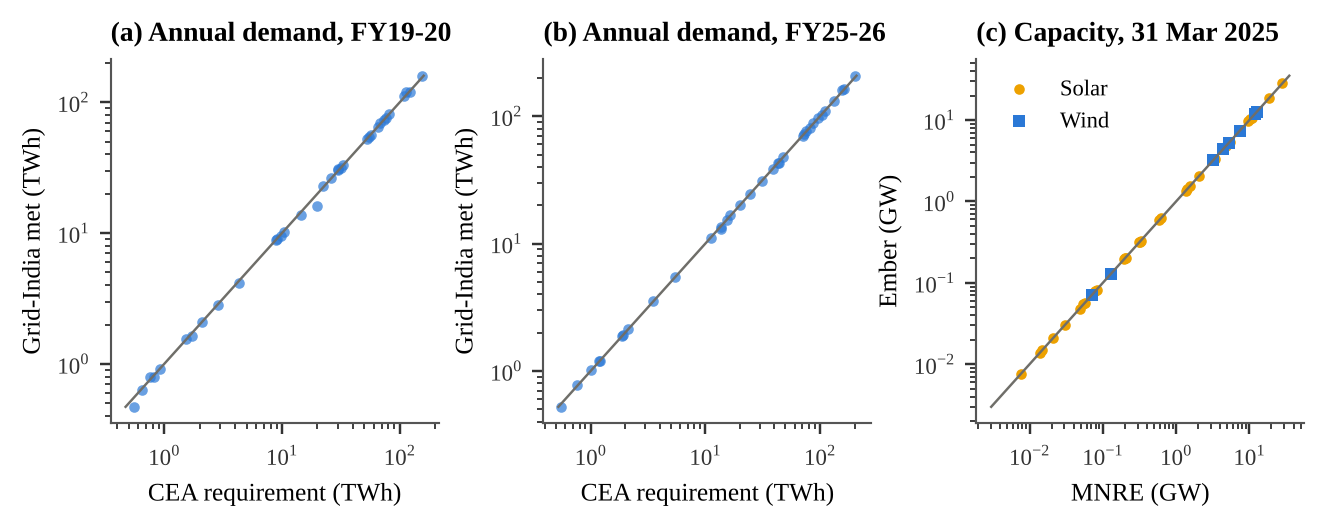
\includegraphics[width=.8\textwidth]{figA_checks.png}
\caption{Cross-checks on log scales. Each dot is a state. The line marks perfect agreement. (a, b) Grid-India energy met against CEA requirement. (c) Ember capacity against MNRE's official table.}
\end{figure}



\section{4. Methodology}
\textbf{Approach.} The questions are descriptive and the sample is small, so we use simple measures that can be checked by hand, and clustering only at the end. No causal model is attempted.

\textbf{Windows.} ``Early'' is FY2019-20 and FY2021-22, skipping COVID-hit FY2020-21. ``Recent'' is FY2023-24 and FY2024-25, the last two full years in Ember. Two years are averaged in each window because one year can mislead: CEA says FY2025-26 demand came in 7.7\% under forecast because of unusual summer weather \cite{lgbr2627}.

\textbf{SQ1 measures.} Growth is the compound yearly rate of energy met. Per capita use divides energy met by population, grown at a steady rate between 2011 and 2026. It includes losses, since it is energy met and not metered sales.
\begin{itemize}
\item Seasonal swing = highest monthly average of daily energy / lowest monthly average, within a year.
\item Flatness = average daily energy / highest daily energy, within a year.
\item Load factor = annual MU $\times$ 1000 / (hours in year $\times$ peak MW), using CEA figures.
\item Peak month = month with the highest value in the window's average seasonal pattern.
\item Seasonal strength from STL decomposition \cite{stl} of log daily average energy with a 12-month period. Values near 1 mean a strong repeating pattern.
\item Shape similarity = average correlation between the monthly shapes of every pair of the 23 largest states.
\end{itemize}
Our plan used monthly MW peaks for swing. We switched to energy because MW peaks were not available for early years, whereas daily energy is complete. Flatness tracks the MW load factor closely (Spearman 0.81 across states in FY2025-26). Changes between windows are tested with a Wilcoxon signed-rank test. A log-log regression of per capita use on per capita GSDP shows which states use more or less than income predicts.

\textbf{SQ2 measures.} Capacity factor (CF) = generation / (average capacity $\times$ hours). Seasonal match is the correlation between the 12-month profile of solar plus wind and the 12-month profile of demand, in energy per day, over the recent window, for the 18 units where solar and wind cover over 1\% of demand. Coverage is solar plus wind generation as a share of demand. Net position = scaled generation / demand. Ember generation is about 7 to 8\% higher than energy met nationally, since it is measured before plant use and some losses, so generation is scaled each year (0.926 in FY2024-25) to make the national balance equal 1. A value above 1 means a net exporter.

\textbf{What-if 1, consumption mix.} Assumptions: (a) each month a state first uses its own generation; (b) any shortfall comes from a national pool made of all states' surplus, in proportion; (c) contracts, line limits and losses are ignored; (d) carbon intensity uses Ember's IPCC factors \cite{ipcc}. We repeat it with annual balancing and with imports drawn first from the state's own region.

\textbf{What-if 2, hidden rooftop output.} Missing solar generation = rooftop and off-grid capacity $\times$ an assumed 13 to 17\% CF. The range is our assumption, a little below the utility-scale values we measure.

\textbf{What-if 3, coal plateau and coal paths.} Assumptions: demand grows 4.0, 5.5 or 6.5\% a year from FY2024-25; new solar and wind runs at 17, 18.5 or 20\% CF (the fleet average was 18.5\%); new hydro, nuclear, storage losses and curtailment are ignored; seasonal timing is ignored, so the need is a lower bound. Coal paths to FY2029-30 use 5.5\% growth, 18.5\% CF and fixed yearly additions of 28, 45, 62 or 80 GW, with coal covering whatever is left.

\textbf{SQ3 method.} Each state in each window gets nine size-free features: coal, hydro and solar-plus-wind shares; log$_2$ net position; log per capita use; demand growth; yearly gain in solar-plus-wind share; swing; flatness. Shares use the larger of scaled generation and demand as the base, otherwise a territory making only 9 GWh, all solar, would count as ``100\% solar'' (Chandigarh's real case). Features are clipped at the 2nd and 98th percentiles and standardised. PCA finds the main directions of difference. K-means groups the 66 rows, with Ward clustering as a second opinion. We picked k using silhouette scores \cite{silhouette} and bootstrap stability \cite{hennig}: states are resampled 300 times with both windows, and each original group is compared with its closest match. Resampling is by state because a state's two rows are not independent.

\section{5. Results and insights}
\subsection{5.1 National picture: capacity moved, energy mostly did not}
Solar capacity tripled from 34.6 GW to 105.6 GW between March 2020 and March 2025, and wind rose from 37.7 GW to 50.0 GW. Figure 2 shows what this delivered. Generation in our panel rose by 440 TWh. Coal supplied 338 TWh of that (77\%) and solar and wind 112 TWh (26\%), while hydro and gas fell. Coal's share went from 71.9\% to 73.1\%. Coal capacity rose only 8\%, to 221.8 GW, so the extra energy came from running existing plants harder: the national coal CF rose from 55.7\% to 69.5\%. Carbon intensity of generation was 614 gCO$_2$e/kWh in FY2019-20 and 616 in FY2024-25.

\begin{figure}[!htbp]\centering
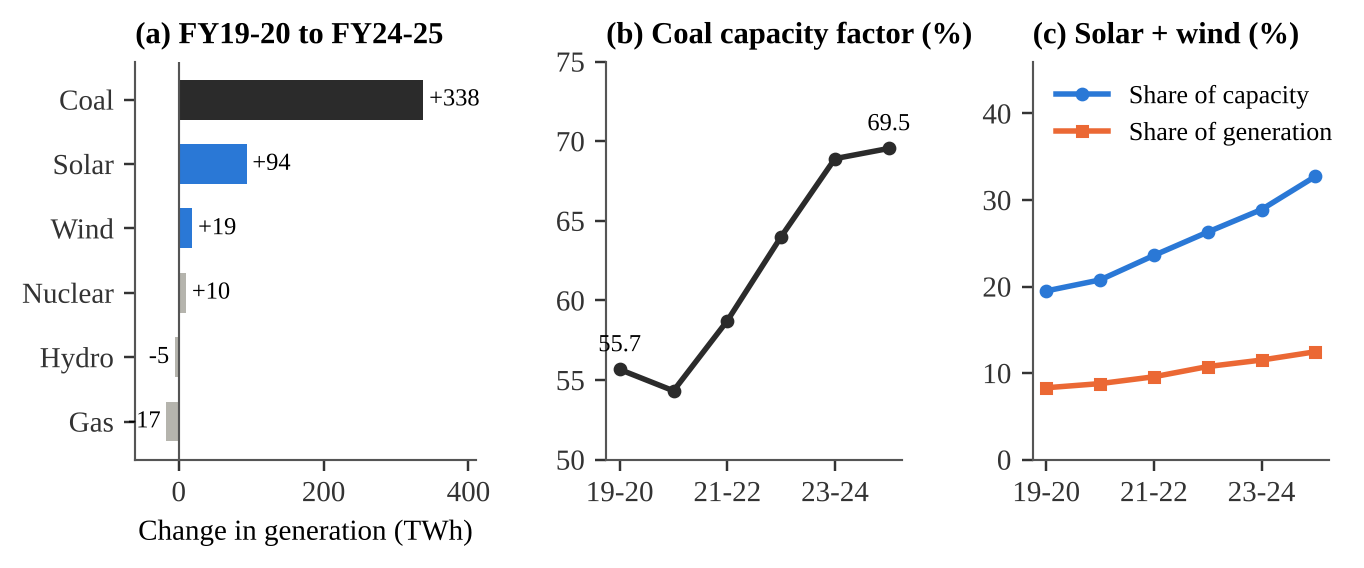
\includegraphics[width=.9\textwidth]{fig1_national.png}
\caption{National supply, FY2019-20 to FY2024-25. Capacity shares in (c) are at year end. Sources: Ember, our calculations.}
\end{figure}

Figure 3a shows that this is not one or two states. Coal CF rose in 15 of the 17 coal states. Odisha (81.8\%), Chhattisgarh (80.2\%) and Jharkhand (79.5\%) now run near their practical limit. The biggest jumps were in Haryana (+30.3 points), Odisha (+28.5), Punjab (+25.6) and Karnataka (+24.7). Only Telangana ($-7.4$) and Gujarat ($-0.4$) fell. At the same time, energy not supplied fell from 0.38\% of demand in FY2019-20, and 0.44\% in FY2022-23, to 0.02\% in FY2025-26 (Figure 3b). The system now meets almost all demand, and it does so mainly by burning more coal.

\textbf{What this means for the grid.} So far the transition has added clean energy on top of coal rather than replacing it. Demand growth has outrun clean additions, and coal plants have much less spare room than five years ago, which raises the risk of shortages in a hot year with a weak monsoon.

\begin{figure}[!htbp]\centering
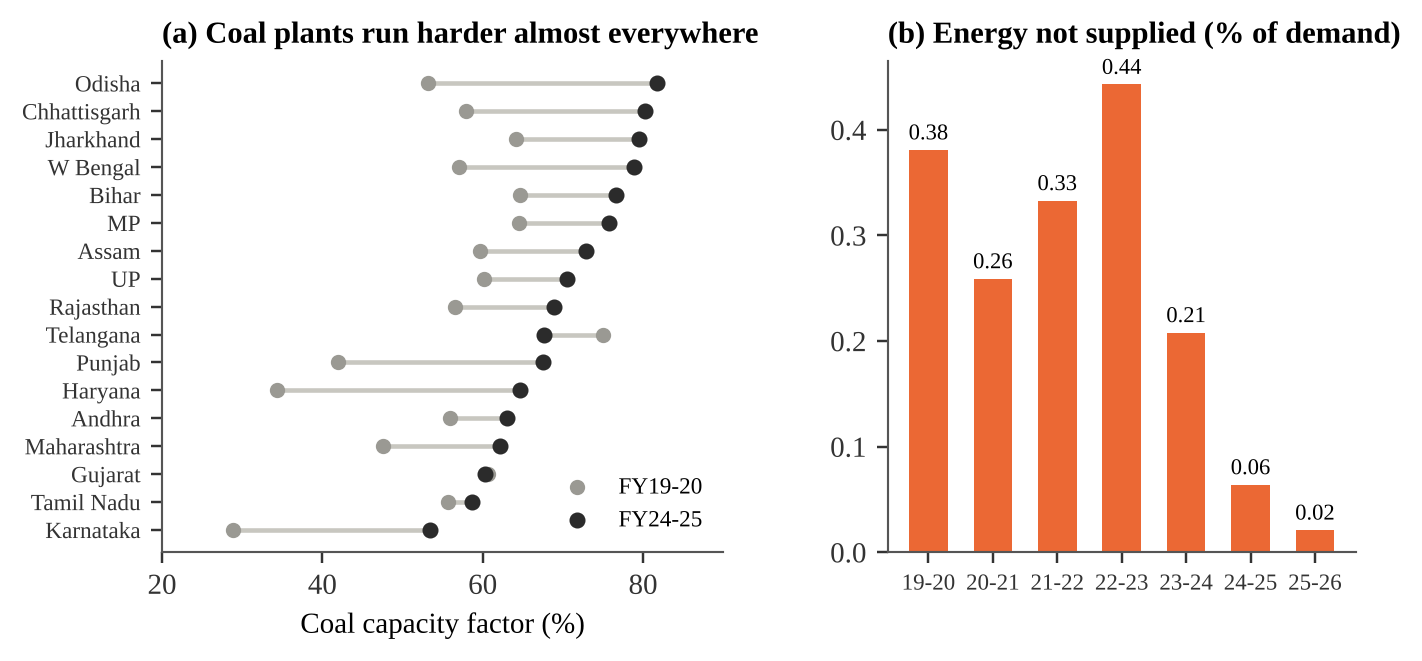
\includegraphics[width=.85\textwidth]{figJ_coalcf.png}
\caption{(a) Coal capacity factor by state, 17 states with over 500 MW of coal. (b) All-India energy shortage from Grid-India daily data. Sources: Ember, Grid-India.}
\end{figure}

\subsection{5.2 SQ1: Demand level differs widely, monthly shape is steady}
Energy met across the 33 units grew from 1,296 TWh in FY2019-20 to 1,689 TWh in FY2024-25, or 5.4\% a year, then only to 1,700 TWh in the mild FY2025-26. Among the 23 units above 10 TWh, growth ranged from 3.0\% (Delhi) and 3.1\% (Tamil Nadu) to 7.2\% (Bihar) and 7.0\% (Rajasthan) (Figure 4a). The fastest growers are poorer or farm-heavy states, while the slowest are the richer, more urban ones.

\begin{figure}[!htbp]\centering
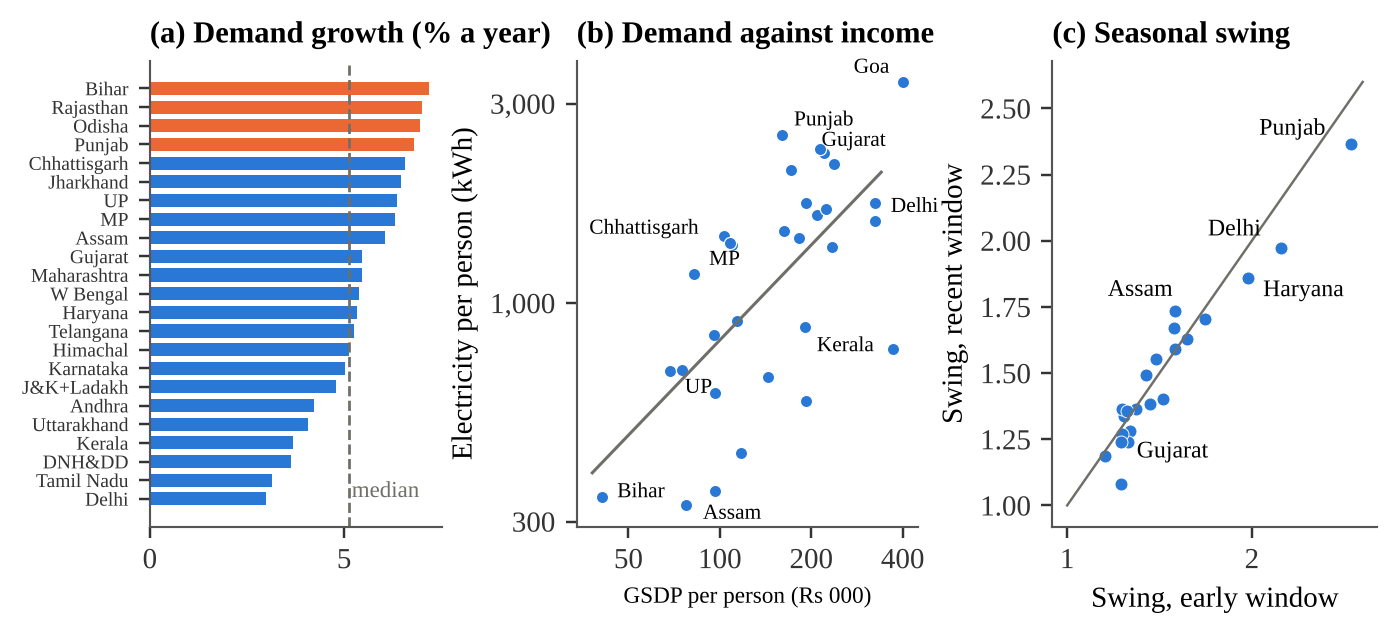
\includegraphics[width=.95\textwidth]{figB_growth.png}
\caption{(a) Compound yearly growth of energy met, FY2019-20 to FY2024-25, 23 units above 10 TWh. (b) Electricity per person against GSDP per person, FY2024-25, 31 units, log scales, with fitted line. (c) Seasonal swing in the early and recent windows. Points near the line did not change.}
\end{figure}

Use per person is far more unequal: 2,529 kWh in Punjab, 2,332 in Telangana and 2,149 in Gujarat, but 343 in Bihar and 355 in Assam, against 1,201 nationally. Income explains part of this. Across 31 units, a 1\% rise in GSDP per person goes with a 0.76\% rise in electricity per person ($R^2=0.43$, Figure 4b). The gaps from this line are telling. Punjab uses 118\% more than its income predicts and Madhya Pradesh 67\% more, which fits heavy farm pumping, though our data cannot separate sectors. Assam (55\% less) and Kerala (34\% less) sit below the line. Bihar has a long way to go, so its demand growth is unlikely to slow soon.

\begin{figure}[!htbp]\centering
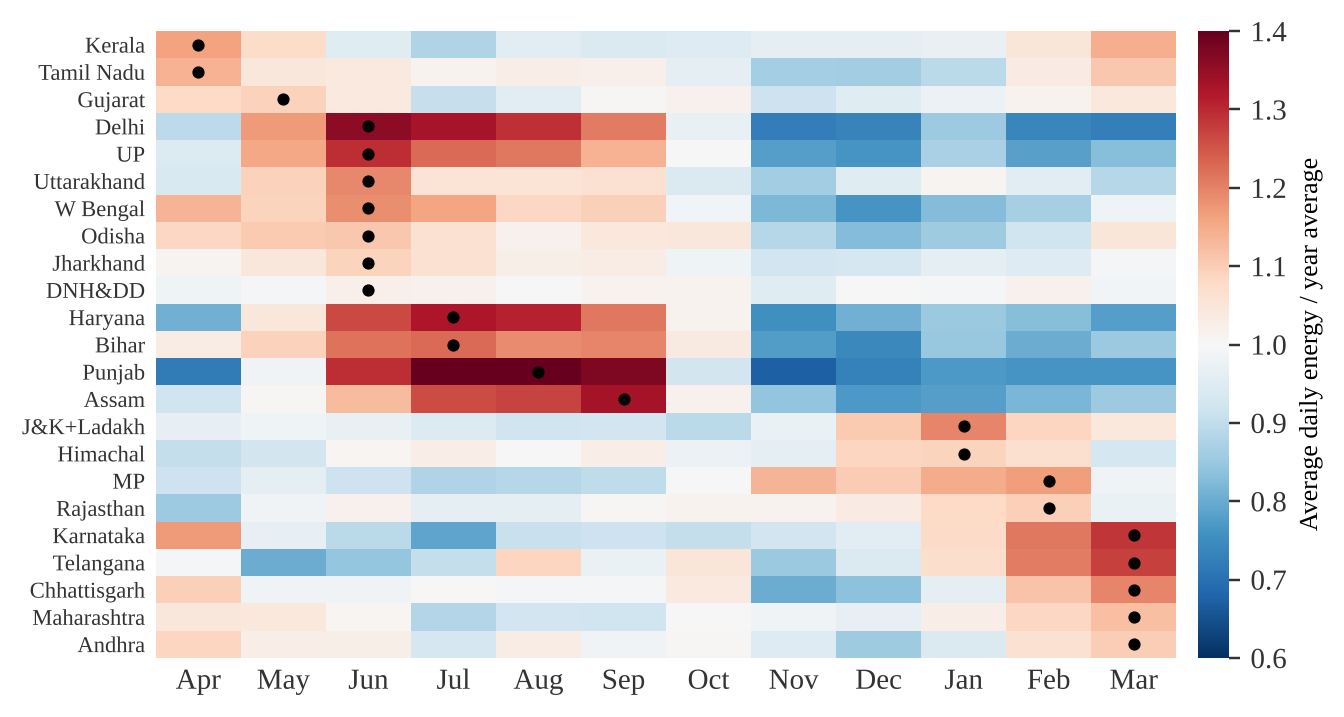
\includegraphics[width=.72\textwidth]{fig3_heatmap.png}
\caption{Seasonal shape of the 23 largest units, FY2023-24 and FY2024-25. Red months are above the state's yearly average. Black dots mark the peak month. Source: Grid-India, our calculations.}
\end{figure}

\textbf{Shape.} Figure 5 shows that India runs on several demand calendars at once. The northern plains and eastern states peak in June to September, with Punjab, Delhi and Haryana showing the strongest swings (2.37, 1.97 and 1.86). The southern states, Maharashtra and Chhattisgarh peak in March or April, Rajasthan and Madhya Pradesh in February (rabi irrigation is the likely reason), and Himachal Pradesh and J\&K in January. Gujarat (1.24) and Maharashtra (1.27) are flat by comparison. STL seasonal strength is highest in Assam and Punjab (0.93) and Bihar (0.90), with a median of 0.74.

\textbf{Is the shape changing?} At state level, hardly at all (Figure 4c). Median swing went from 1.34 to 1.37, with 16 units up and 17 down (Wilcoxon $p=0.72$). Median flatness went from 0.770 to 0.767 ($p=0.68$). Peak month changed in 18 of 33 units, but most moves are one month, which is within normal weather noise. The clearest shift is in the east: Jharkhand and West Bengal moved from April to June, and Odisha from August to June. One quieter change is that state calendars are drifting apart: the average correlation between the monthly shapes of the 23 large states fell from 0.25 to 0.15. That helps the national grid, because states peaking at different times can share capacity.

\begin{figure}[!htbp]\centering
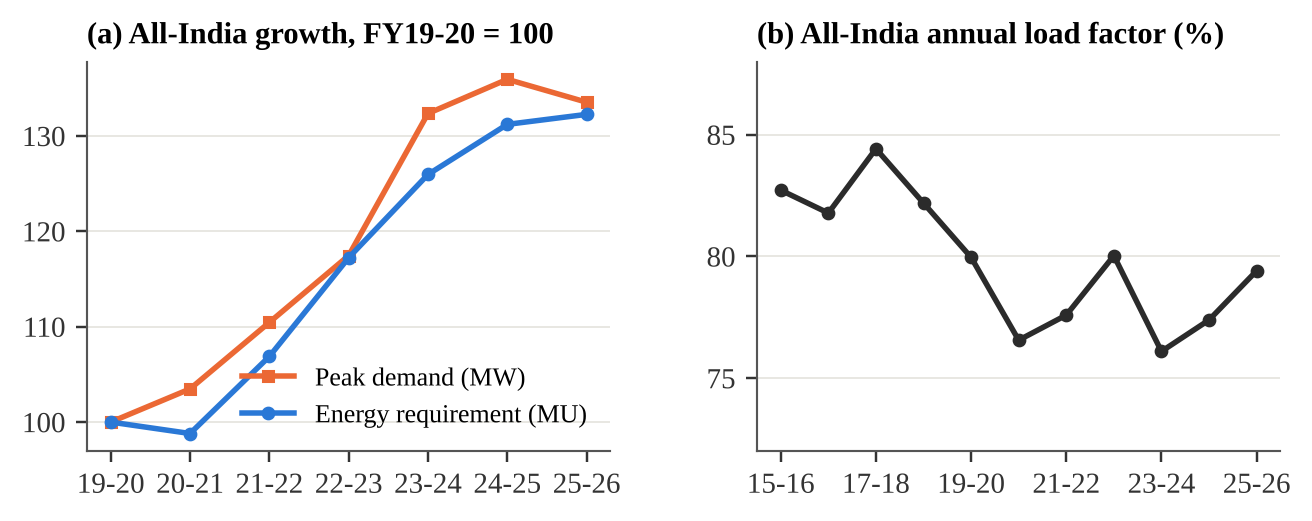
\includegraphics[width=.8\textwidth]{fig2_load.png}
\caption{All-India energy requirement, peak demand and load factor. Source: CEA \cite{lgbr2627}, our calculations.}
\end{figure}

\textbf{The change is in the peak.} National peak demand grew 6.3\% a year from FY2019-20 to FY2024-25, against 5.6\% for energy (Figure 6). The national load factor was above 80\% until FY2018-19 and has mostly been 76 to 80\% since. Yet daily flatness barely moved nationally (0.856 to 0.852), and the ratio of summed state peak days to the national peak day shows no trend (1.14 to 1.13). If days and seasons are not getting peakier and states are not lining up more, the likely cause is a sharper peak within the day, which fits growing cooling load. Part of the faster peak growth may also come from the drop in shortages, since less demand is now cut at peak times. Monthly data cannot prove either point. The FY2025-26 rebound to 79.4\% came with a weak summer, and the system then hit 270.8 GW on 21 May 2026, very close to CEA's 271.6 GW forecast for the year \cite{lgbr2627,gridindia}.

\subsection{5.3 SQ2: Installed capacity against delivered energy}
\begin{figure}[!htbp]\centering
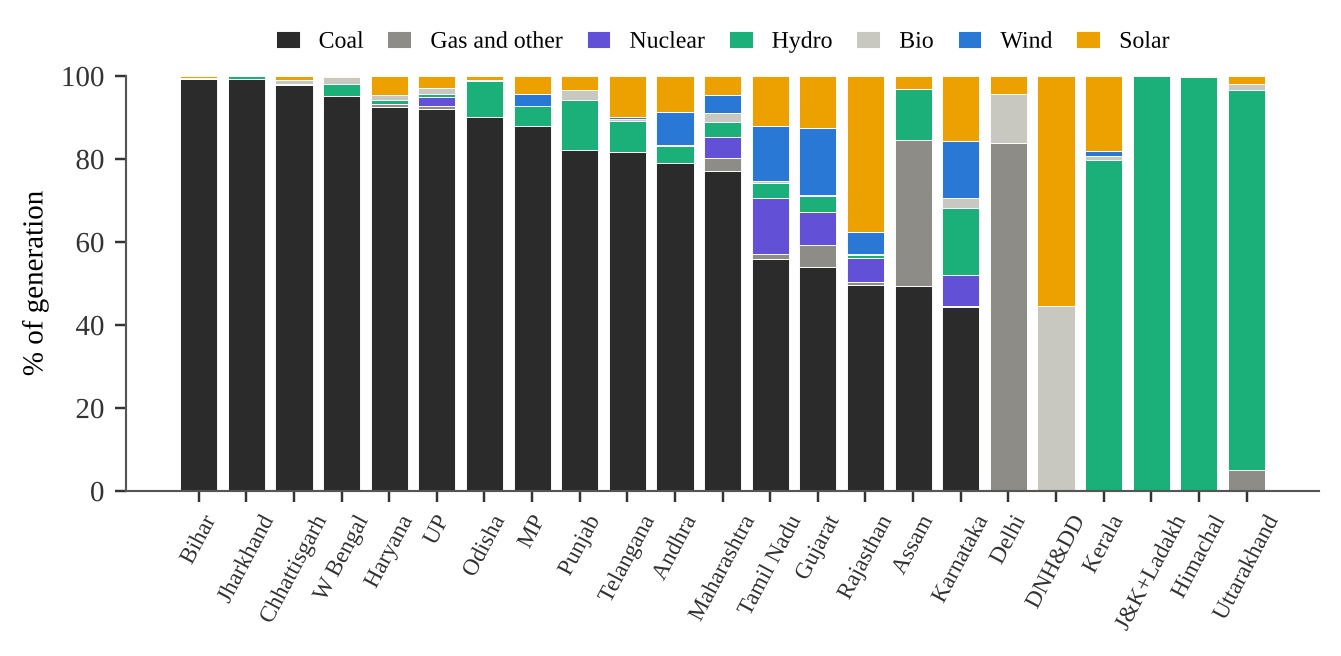
\includegraphics[width=.9\textwidth]{figC_mix.png}
\caption{Generation mix of the 23 largest units, FY2024-25, sorted by coal share. Source: Ember.}
\end{figure}

\textbf{Where the energy comes from.} Figure 7 shows how unequal the supply side is. Twelve of the 23 large units get over 75\% of their generation from coal, and Bihar, Jharkhand and Chhattisgarh over 97\%. Apart from DNH\&DD, whose local generation is tiny, only Rajasthan, Gujarat, Tamil Nadu and Karnataka have solar and wind above a quarter of generation. The hill states, Kerala and J\&K run almost entirely on hydro, Delhi runs on gas (84\%), and Assam on coal and gas.

\textbf{Who added what.} Figure 8 shows the change in generation by state. Four states (Rajasthan, Gujarat, Tamil Nadu and Karnataka) produced 82\% of the extra solar and wind output, and Rajasthan alone 37\%. Six states (Chhattisgarh, Uttar Pradesh, Madhya Pradesh, Odisha, Bihar and Maharashtra) produced 59\% of the extra coal output. Only Rajasthan, Gujarat and Tamil Nadu added more solar and wind than coal, while 18 units added more coal than solar and wind. Even Rajasthan added 19 TWh of coal. Bihar and Uttar Pradesh show up as big coal adders partly because central NTPC plants located there count for the host state.

\begin{figure}[!htbp]\centering
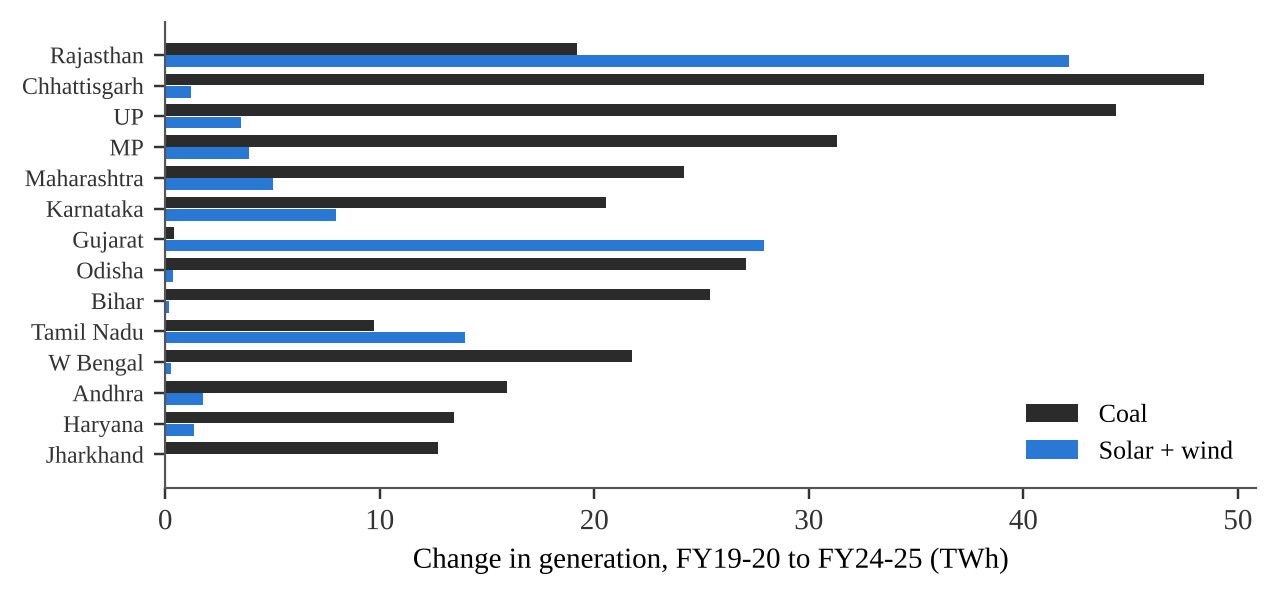
\includegraphics[width=.72\textwidth]{figD_added.png}
\caption{Change in annual generation, FY2019-20 to FY2024-25, 14 units with the largest change. Source: Ember.}
\end{figure}

\begin{table}[!htbp]\small\centering
\caption{Solar and wind in the eight largest units by solar and wind capacity, FY2024-25.}
\begin{tabular}{lrrrrrrr}
\toprule
State & Solar+wind & Share of & Share of & Solar CF & Rooftop & Wind CF & Seasonal\\
 & GW (avg) & capacity \% & generation \% & \% & share \% & \% & match $r$\\
\midrule
Rajasthan & 29.9 & 68.8 & 42.9 & 22.7 & 8.2 & 15.2 & $-$0.30\\
Gujarat & 28.0 & 50.3 & 28.8 & 14.4 & 28.1 & 23.7 & 0.35\\
Tamil Nadu & 20.3 & 49.0 & 25.4 & 19.6 & 9.9 & 17.8 & 0.25\\
Karnataka & 15.7 & 47.5 & 29.3 & 19.9 & 7.6 & 23.4 & $-$0.44\\
Maharashtra & 13.3 & 27.5 & 9.0 & 10.9 & 43.9 & 16.7 & $-$0.57\\
Andhra Pradesh & 8.9 & 30.4 & 16.5 & 19.2 & 7.1 & 20.0 & 0.16\\
Madhya Pradesh & 7.4 & 23.1 & 7.1 & 18.1 & 12.0 & 18.7 & $-$0.22\\
Telangana & 4.9 & 28.6 & 10.3 & 16.4 & 9.9 & n/a & 0.43\\
\bottomrule
\end{tabular}
\end{table}

\textbf{Capacity share overstates energy share.} Nationally, solar and wind were 32.7\% of capacity and 12.5\% of generation in FY2024-25. Table 2 and Figure 9a show the same gap by state: every point sits well below the equal-share line. This is partly physics, since a solar plant runs at about a fifth of its rating. For wind there is real variation (Figure 9b): Gujarat (23.7\%) and Karnataka (23.4\%) against Rajasthan (15.2\%) and Maharashtra (16.7\%). If the four large wind states below the capacity-weighted average of 20.0\% reached it, wind output would rise by only 6.1 TWh, so better use of existing wind plant is not the main lever.

\begin{figure}[!htbp]\centering
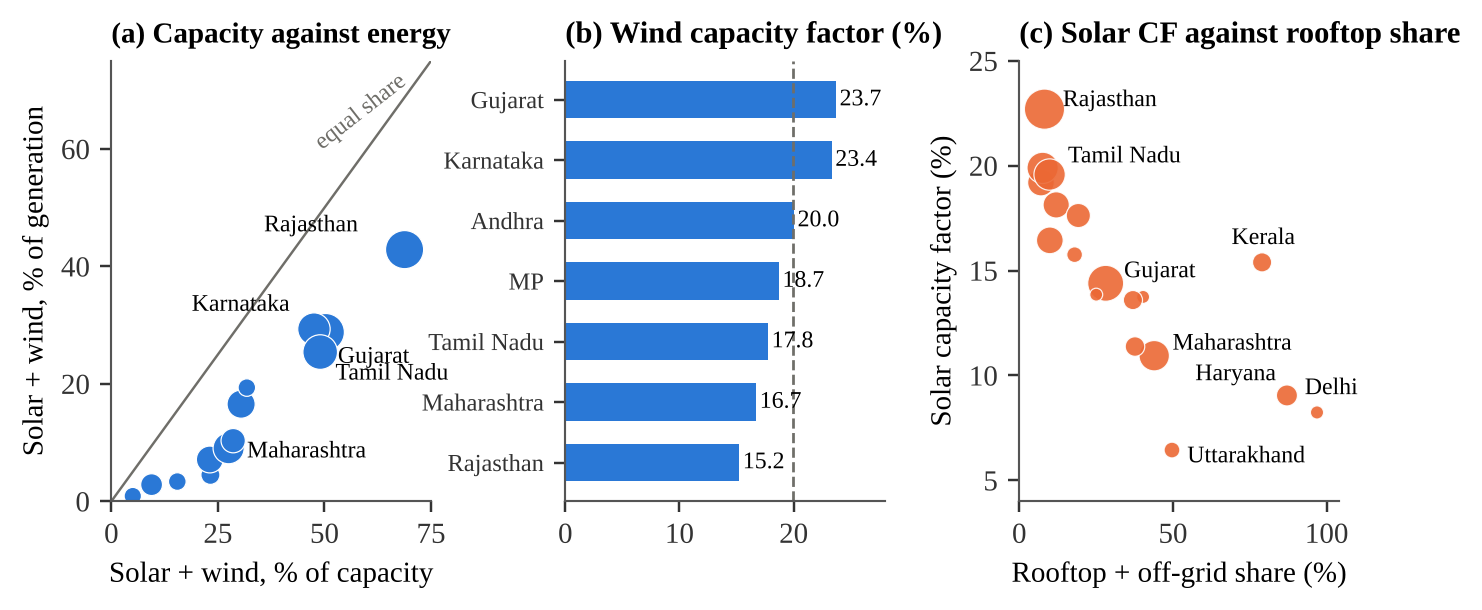
\includegraphics[width=.95\textwidth]{figE_capacity.png}
\caption{FY2024-25. (a) Solar and wind share of capacity against share of generation, units with over 1 GW; marker size shows capacity. (b) Wind capacity factor, states with over 1 GW; dashed line is the capacity-weighted average. (c) Solar capacity factor against rooftop and off-grid share of solar capacity, 18 states with over 200 MW; marker size shows solar capacity.}
\end{figure}

\textbf{A data finding: rooftop output looks largely missing.} Maharashtra's solar CF looks like 10.9\% and Gujarat's 14.4\%, against 22.7\% in Rajasthan. That is not a physical gap. Figure 9c shows that across 18 states with over 200 MW of solar, CF falls steadily as the rooftop share rises (Pearson $-0.76$, $p<0.001$; Spearman $-0.90$). Ember capacity includes rooftop and off-grid plant, but the generation reports seem to capture little of their output. This comes from combining MNRE's official split for 31 March 2025 with Ember's generation. Dividing by non-rooftop capacity alone gives believable values of 18.3 to 24.7\% for 11 of the larger solar states (Maharashtra 19.5\%, Gujarat 20.0\%). It fails for Haryana and Kerala (about 70\%), so some rooftop output is counted there and this is only an approximation. With 18.6 GW of rooftop and off-grid capacity, what-if 2 suggests 21 to 28 TWh a year of unrecorded solar, about 17\% of reported solar output or 1.4\% of demand.



\textbf{Season matters more than the annual average.} Figure 10a shows the national month-by-month supply. Hydro and wind both peak in the monsoon at about 1.8 times their yearly average, while solar peaks in March (1.3 times) and dips in July. Together they produce 1.43 TWh a day in August but only 0.71 in November (Figure 11a). Demand moves far less, from 4.03 to 4.84 TWh a day. Coal takes up the difference, so its share swings from 66\% in August to 78\% in January (Figure 10b). Coal output is highest in March and April, when solar is high but hydro and wind are low and demand is rising.

\begin{figure}[!htbp]\centering
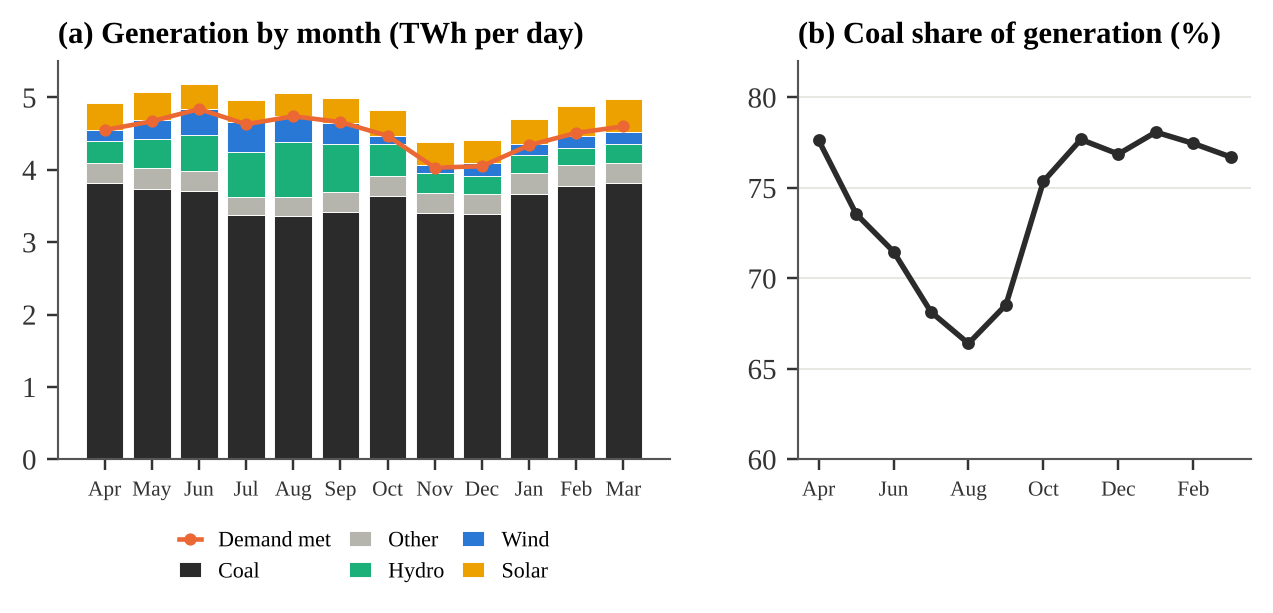
\includegraphics[width=.85\textwidth]{figF_month.png}
\caption{(a) All-India generation by fuel and demand met, in TWh per day, average of FY2023-24 and FY2024-25. (b) Coal share of generation by month. Sources: Ember, Grid-India.}
\end{figure}

\begin{figure}[!htbp]\centering
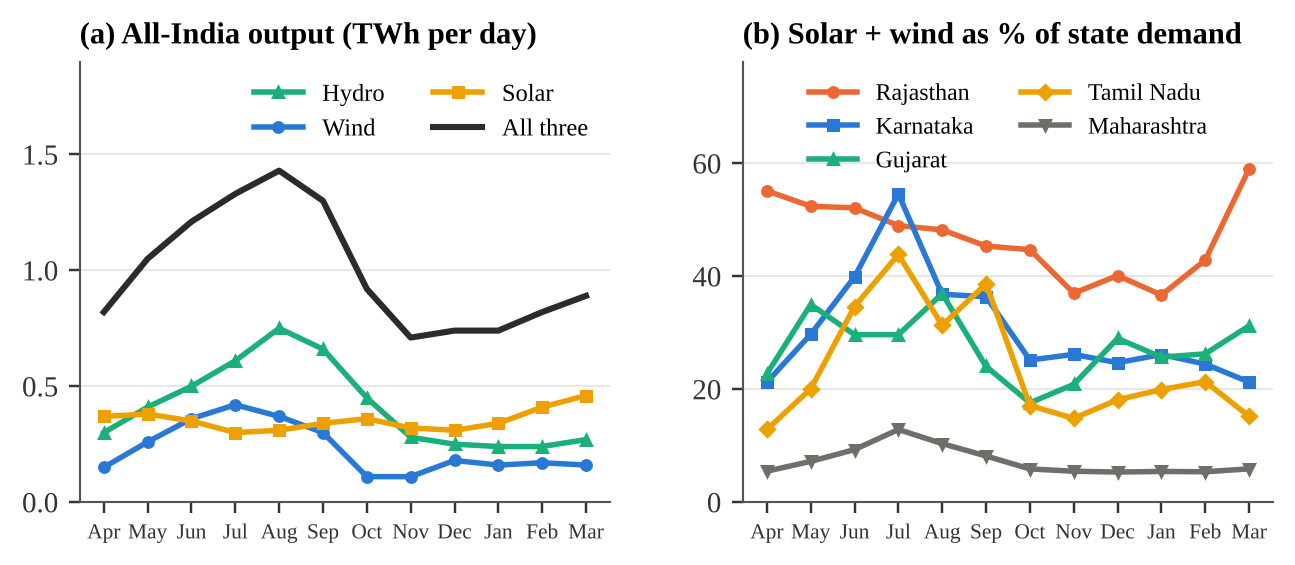
\includegraphics[width=.85\textwidth]{fig5_seasonal.png}
\caption{Seasonal supply, averaged over FY2023-24 and FY2024-25. Sources: Ember, Grid-India, our calculations.}
\end{figure}

The worst fit is in spring, when many western and southern states hit their peak. Karnataka's solar and wind cover 55\% of demand in July but 21\% in its peak month of March, and Tamil Nadu falls from 44\% to 13\% (Figure 11b). Figure 12a puts this side by side: Tamil Nadu covers 24\% over the year but only 13\% in its peak month, and Karnataka 30\% against 21\%. Seasonal match is negative in 8 of 18 states, lowest in Maharashtra ($-0.57$) and Karnataka ($-0.44$) (Figure 12b). Gujarat does better than its peers (35\% coverage in its May peak against 27\% over the year), because its wind is strong in May, its peak month. Rajasthan shows what solar-led supply looks like: coverage stays between 37\% and 59\% all year and is highest in March.

\begin{figure}[!htbp]\centering
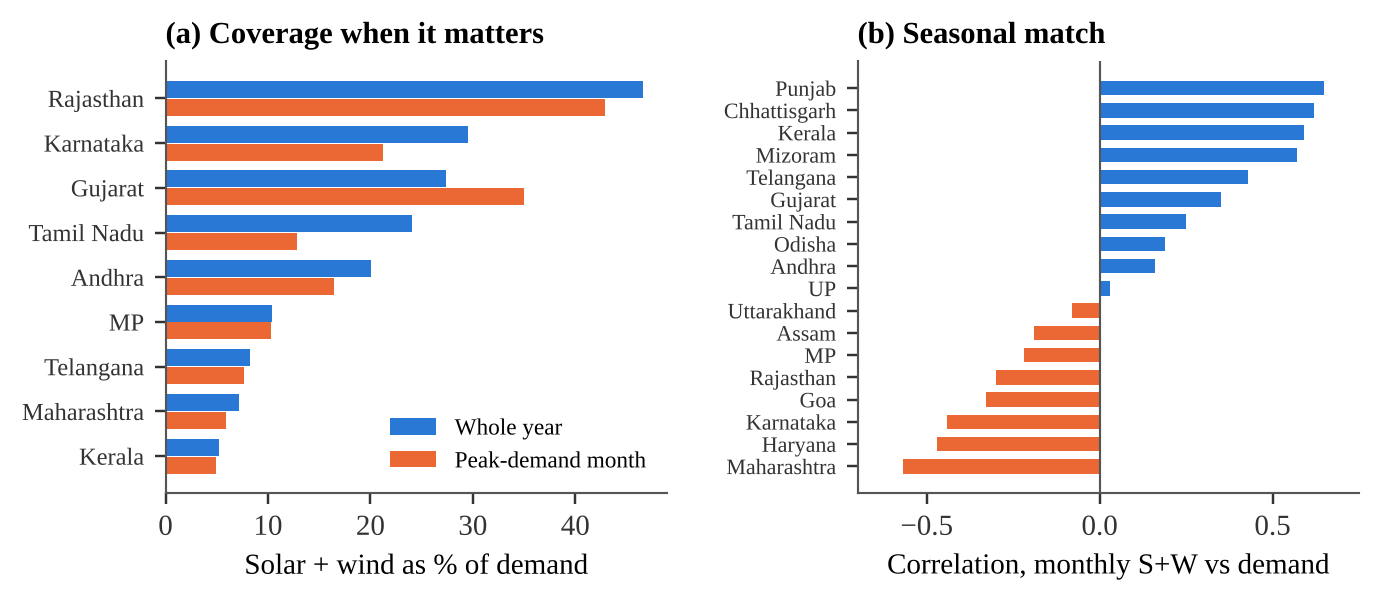
\includegraphics[width=.85\textwidth]{figK_cover.png}
\caption{(a) Solar and wind as a share of demand, over the whole year and in the state's peak-demand month, recent window, states above 5\%. (b) Correlation between monthly solar plus wind and monthly demand, 18 units. Orange: negative.}
\end{figure}

\textbf{Net position changes with the season.} No single dataset shows this, since it needs Ember's generation and Grid-India's demand together. Over the 24 months of the recent window, 14 units were importers in every month and 6 were exporters in every month (Figure 13). The other 13 switched. Uttarakhand was a net exporter in 7 of 24 months and J\&K in 10, all between May and September when hydro is high, and Karnataka in 7, mostly in the monsoon. Chhattisgarh (3.68), Himachal Pradesh (3.03) and Odisha (1.67) are large exporters, while Delhi (0.11), Kerala (0.28), Haryana (0.43) and Punjab (0.48) depend heavily on others. Rajasthan is a small net exporter (1.07), with a surplus in 16 of 24 months.

\begin{figure}[!htbp]\centering
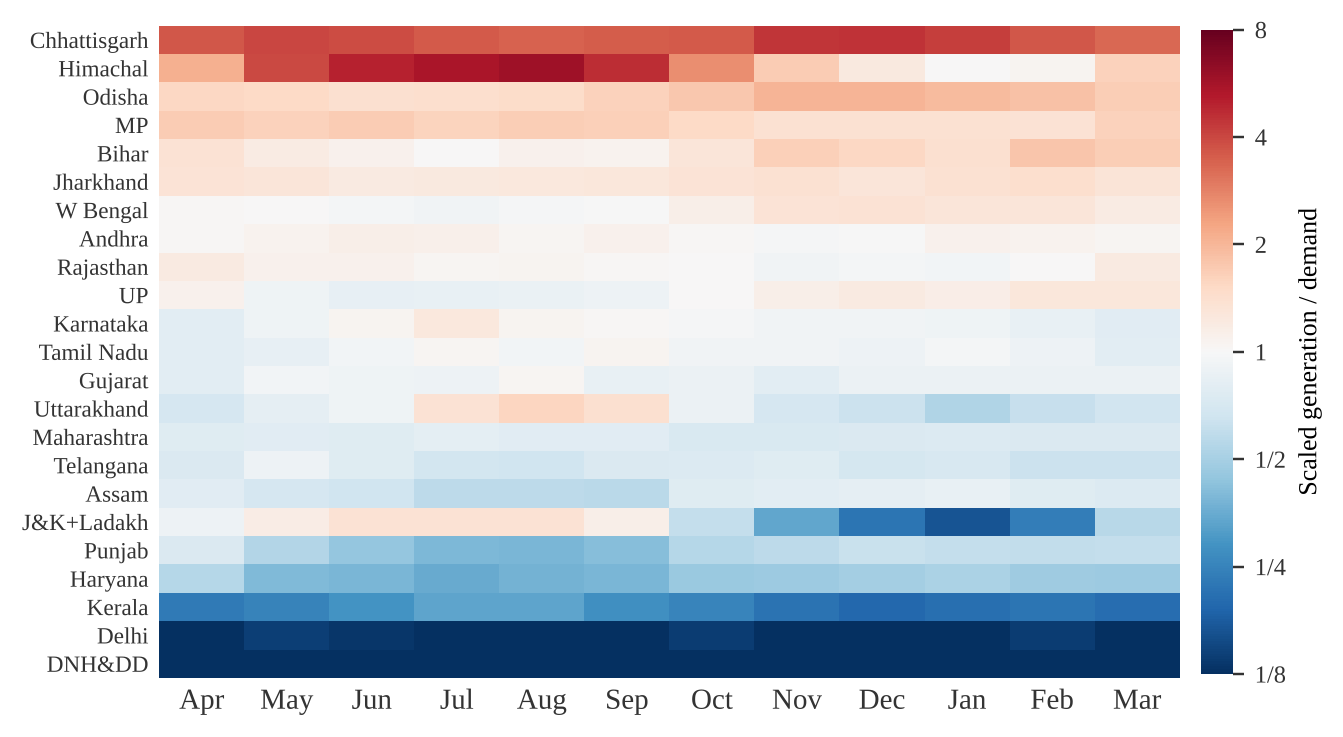
\includegraphics[width=.72\textwidth]{figG_net.png}
\caption{Scaled generation divided by demand, by month, 23 largest units, recent window. Red: net exporter. Blue: net importer. Sources: Ember, Grid-India, our calculations.}
\end{figure}

\textbf{What-if 1: states consume a different mix from what they generate.} Figure 14 compares the two. The gaps are large for importers. Delhi burns no coal locally, yet an estimated 68\% of what it consumes comes from coal, and its carbon intensity rises from 417 to 618 gCO$_2$e/kWh. Kerala goes from 29 to 498, with solar and wind falling from 19\% to 8\% of its mix. J\&K goes from 24 to 296. Goa's local generation is 88\% solar, which means almost nothing, since local plants meet only about 1\% of its demand. Generators barely change: Rajasthan stays at 432 to 433, and Chhattisgarh at 805. Among the 23 large units, the spread (standard deviation) falls from 284 to 206 gCO$_2$e/kWh, so states are more alike in what they consume than in what they generate.

The result is stable to how we run it. Annual balancing instead of monthly moves the median state by 4 gCO$_2$e/kWh, and importing from the region first moves it by 6, though one state moves by 116. So the ranking of the big importers can be trusted more than the exact numbers.

\begin{figure}[!htbp]\centering
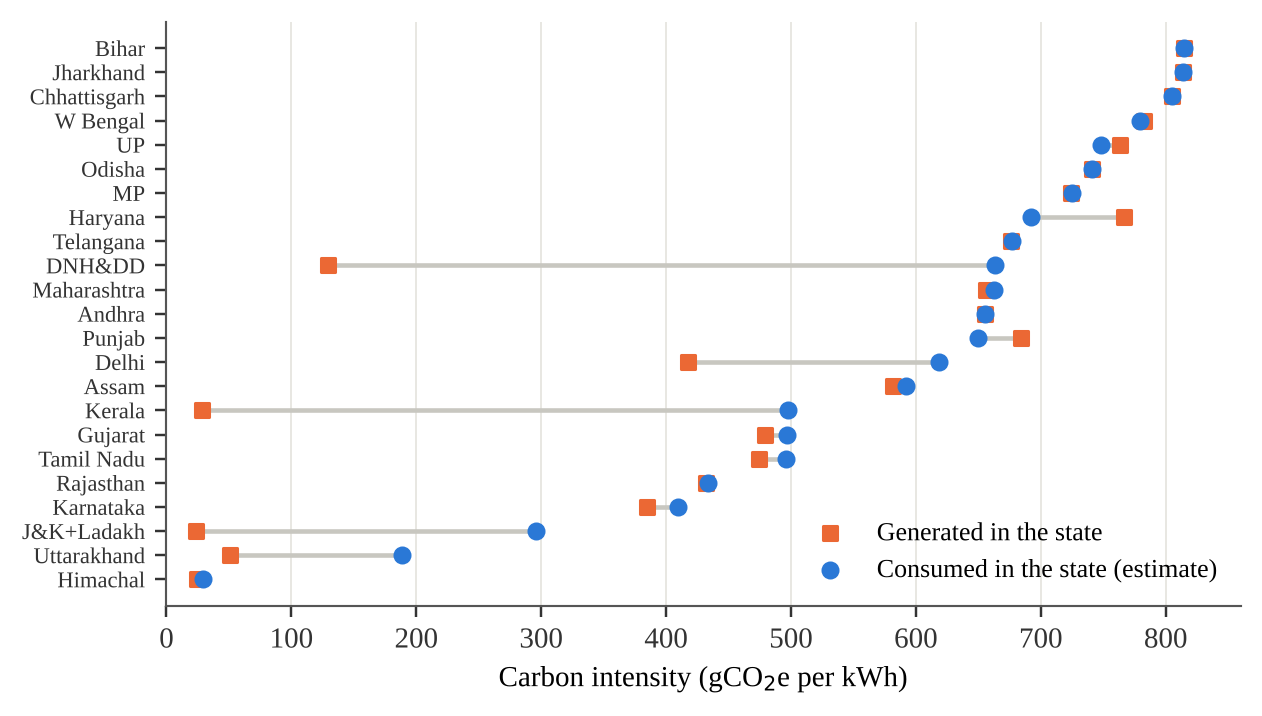
\includegraphics[width=.62\textwidth]{fig6_consumption.png}
\caption{Carbon intensity of electricity generated in a state against our estimate for electricity consumed there, 23 largest units, FY2024-25. The consumed values are a scenario under the stated assumptions.}
\end{figure}

\textbf{What-if 3: what would stop coal growing?} Table 3 shows that at central values India needs about 62 GW of new solar and wind every year just to cover demand growth, with a range of 42 to 80 GW. The fleet added 28.0 GW in FY2024-25, a record in our panel, and 16.7 GW a year on average over five years (Figure 15a). So even the fastest year is less than half the central need and below the lowest cell of that table. Figure 15b turns this into coal output. At the current 28 GW a year, coal generation rises from 1,332 TWh to about 1,665 TWh by FY2029-30, a 25\% increase. At 62 GW it stays nearly flat (1,390 TWh), and only at 80 GW does it start to fall (1,244 TWh). This explains the finding in Section 5.1, and it shows that even doubling the current pace would leave coal output growing.

\begin{table}[!htbp]\small\centering
\caption{New solar and wind needed per year (GW) so that coal stops growing, under what-if 3.}
\begin{tabular}{lrrrr}
\toprule
Demand growth & TWh needed a year & CF 17\% & CF 18.5\% & CF 20\%\\
\midrule
4.0\% & 72.9 & 49.0 & 45.0 & 41.6\\
5.5\% & 100.3 & 67.3 & 61.9 & 57.2\\
6.5\% & 118.5 & 79.6 & 73.1 & 67.6\\
\bottomrule
\end{tabular}
\end{table}

\begin{figure}[!htbp]\centering
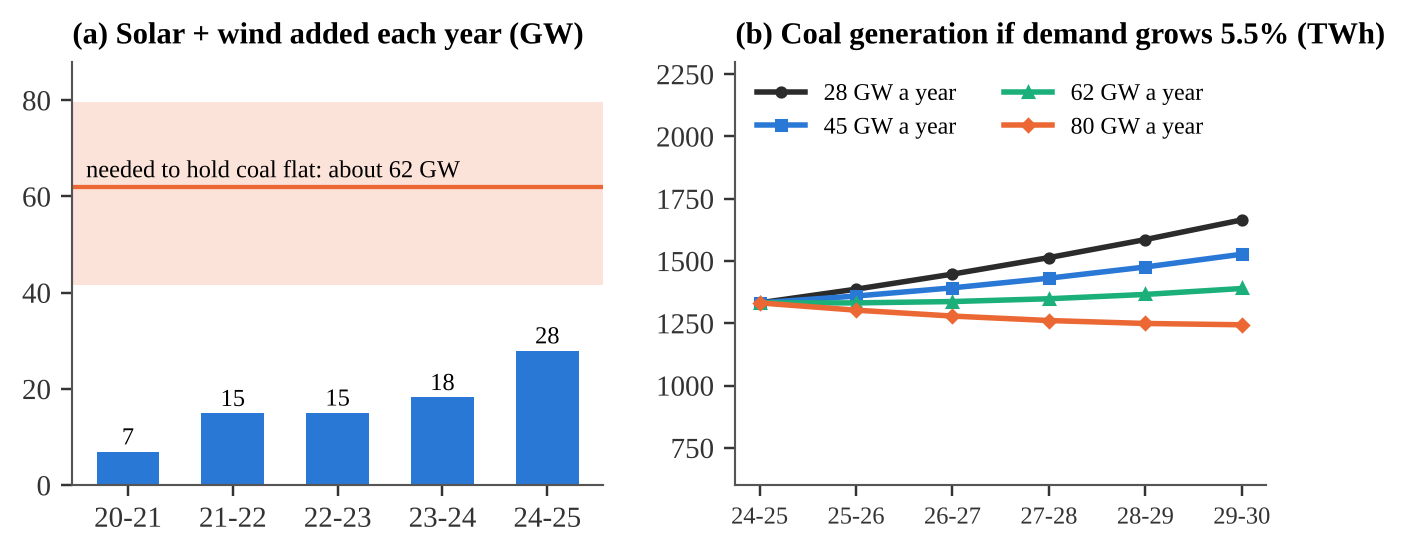
\includegraphics[width=.82\textwidth]{figH_whatif.png}
\caption{(a) Solar and wind capacity added each year against the range needed to hold coal flat (shaded, from Table 3). (b) Coal generation to FY2029-30 under four fixed yearly addition rates, with demand growing 5.5\% a year.}
\end{figure}

\subsection{5.4 SQ3: A typology of state transitions}
PCA shows there is no single ``transition score''. Five components are needed to reach 80\% of the variance, and the first two hold 26\% and 19\%. PC1 rises with solar and wind share (loading 0.50), recent solar-and-wind gains (0.46) and flat load (0.44), and falls with hydro ($-0.28$) and swing ($-0.32$). PC2 rises with net export (0.68) and coal share (0.40) and falls with use per person ($-0.50$), so it separates poorer exporting states from rich importers (Figure 16).

\begin{figure}[!htbp]\centering
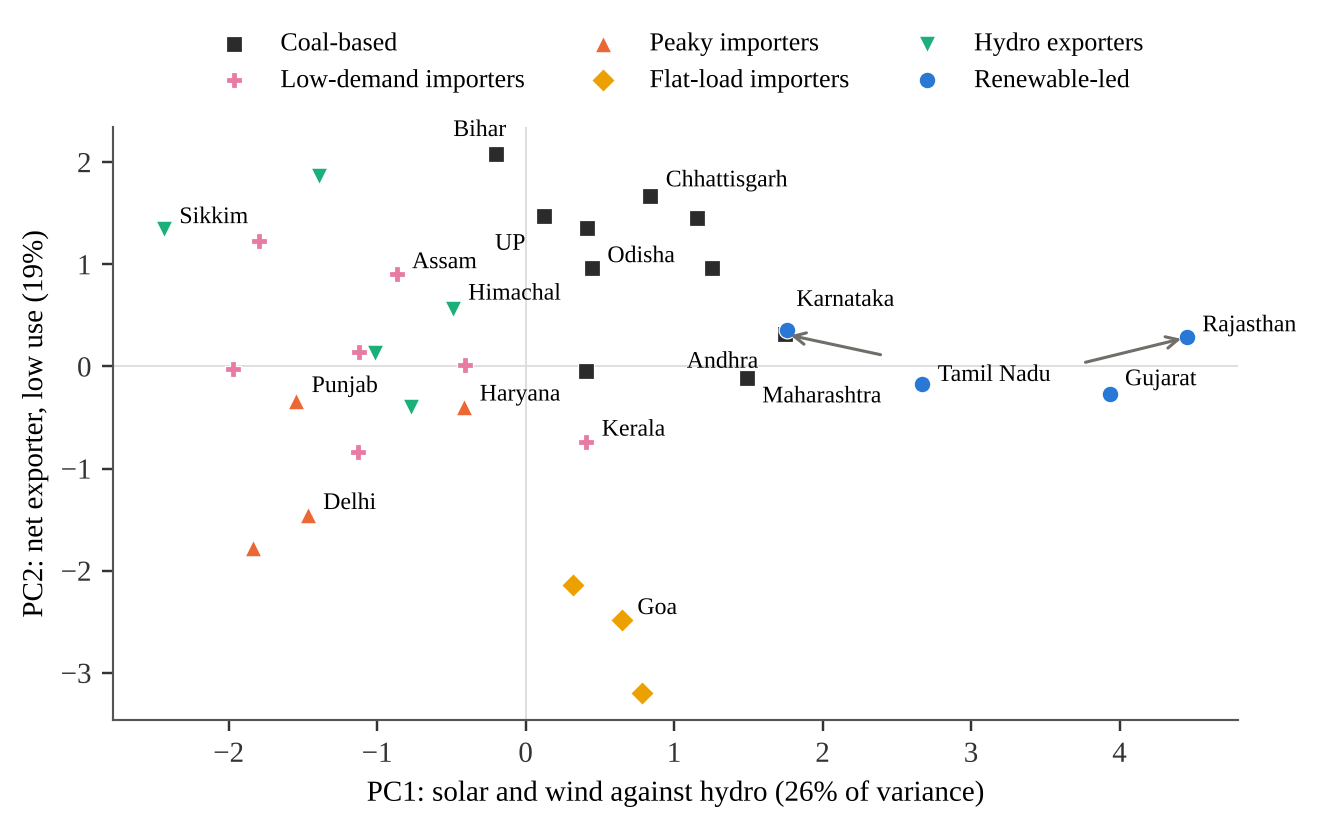
\includegraphics[width=.62\textwidth]{fig7_pca.png}
\caption{States on the first two principal components, recent window. Arrows show the move from the early window for Rajasthan and Andhra Pradesh.}
\end{figure}

We chose k = 6, which gives the best silhouette (0.349) and the strongest weakest-group stability (Jaccard 0.697), with a bootstrap ARI of 0.788 (Figure 17a). A silhouette of 0.35 means the groups are real but not sharply separated, so borderline states matter. The result does not depend on DVC at all: both alternative splits give identical groups (ARI 1.0). Dropping any one feature gives ARI between 0.70 and 1.00. Ward agrees at 0.78, and using only the 23 large units with five groups agrees at 0.86. Table 4 and Figure 17 give the typology.

\begin{figure}[!htbp]\centering
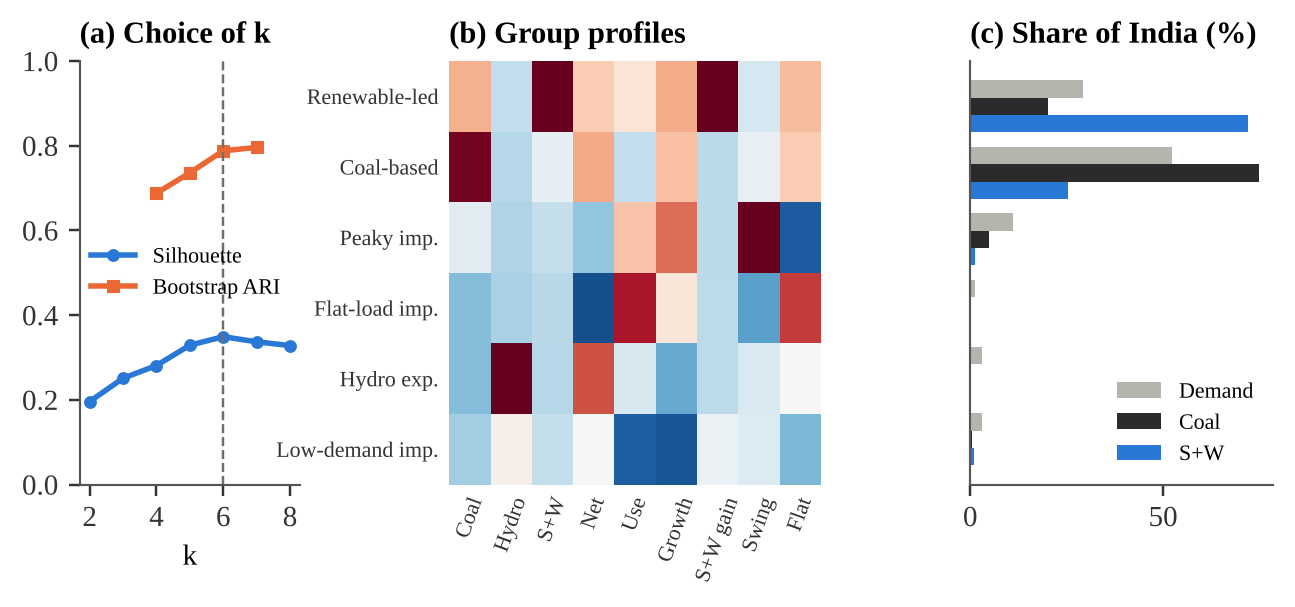
\includegraphics[width=.85\textwidth]{figI_groups.png}
\caption{(a) Silhouette and bootstrap ARI for k = 2 to 8. (b) Average features of each group, standardised across groups (red high, blue low). (c) Each group's share of national demand, coal output and solar plus wind output, FY2024-25. Rows in (b) and (c) match.}
\end{figure}

\begin{table}[!htbp]\footnotesize
\caption{Typology of state transitions, recent window. Demand, coal and solar+wind columns are shares of the national total. Swing is the group average.}
\begin{tabularx}{\textwidth}{>{\raggedright\arraybackslash}p{1.9cm}>{\raggedright\arraybackslash}p{4.1cm}rrrrY}
\toprule
Group & Members & Dem. & Coal & S+W & Swing & Main challenge\\
\midrule
Renewable-led & Gujarat, Karnataka, Rajasthan, Tamil Nadu & 29\% & 20\% & 72\% & 1.40 & Seasonal fit and curtailment; spring peaks in the south\\
Coal-based & Andhra, Bihar, Chhattisgarh, Jharkhand, MP, Maharashtra, Odisha, Telangana, UP, W Bengal & 52\% & 75\% & 25\% & 1.45 & Fast demand growth with low renewable share; holds 64\% of population\\
Peaky importers & Chandigarh, Delhi, Haryana, Punjab & 11\% & 5\% & 1\% & 2.08 & Very sharp seasonal peaks and import dependence\\
Flat-load importers & DNH\&DD, Goa, Puducherry & 1\% & 0\% & 0\% & 1.20 & Almost full import dependence; industrial load\\
Hydro exporters & Arunachal, Himachal, J\&K+Ladakh, Sikkim, Uttarakhand & 3\% & 0\% & 0\% & 1.41 & Winter shortfall; rainfall risk; hold 50\% of hydro output\\
Low-demand importers & Assam, Kerala, Manipur, Meghalaya, Mizoram, Nagaland, Tripura & 3\% & 0\% & 1\% & 1.42 & Low use, thin local supply\\
\bottomrule
\end{tabularx}
\end{table}



\textbf{Almost nobody changed group.} Of 33 units, only Andhra Pradesh moved. It left the renewable-led group for the coal-based group, as its solar-and-wind share slipped from 18.8\% to 17.7\% and coal rose from 73\% to 79\%. Rajasthan moved the furthest along the renewable path, doubling its share from 20.7\% to 41.5\%, but stayed in the same group. Karnataka could follow Andhra Pradesh. It is the least secure member of its group, and its coal share rose from 35\% to 44\% while its solar-and-wind share stayed near 28\%, because new demand was met mainly by coal. Going the other way, Maharashtra is the best placed of the large coal-based states: its coal share fell from 62\% to 59\% and the renewable-led group is its nearest alternative, but its solar-and-wind share is still only 6.6\%.

In short, a group with 29\% of demand produces 72\% of India's solar and wind, while a group with 52\% of demand and 64\% of the population produces 25\%. The transition is concentrated, and the state pattern has been sticky over five years. States will not drift into a cleaner group on their own. The coal-based group's demand grew 6.9\% a year on average in the recent window, so this is where the climate result will be decided.

\section{6. Discussion and limitations}
\textbf{What the data cannot tell us.}
\begin{itemize}
\item \textbf{Hours.} Monthly and daily state data cannot show the evening ramp or solar curtailment. Our claim that peaks are sharpening within the day is an inference, and hourly demand data could test it.
\item \textbf{Cause.} We do not separate weather, income, tariffs or farm policy. The irrigation and cooling explanations are likely but untested, because we have no sector data. Weather years differ, and two windows only partly deal with that.
\item \textbf{Real power flows.} The consumption mix is a scenario. Long-term contracts decide who buys from whom, so a state contracted to hydro or to a specific coal plant will differ from the pool. Line limits and losses are ignored. Results for one state could change a lot, as the 116 gCO$_2$e/kWh case shows.
\item \textbf{Captive and behind-the-meter supply.} Captive plants are outside Ember's state data, so coal use in industrial states is understated. Rooftop output is mostly unmeasured, which understates both solar generation and true demand. Maharashtra and Gujarat are most affected.
\item \textbf{Plant location.} Central plants count for the state that hosts them, so Bihar and Uttar Pradesh look like bigger coal producers, and better net exporters, than their own DISCOMs' contracts would suggest.
\end{itemize}

\textbf{Possible biases.} Ember's generation is 7 to 8\% above energy met, and we scaled all states by one factor, though plant use and losses differ by state. In early years energy met is below true demand in J\&K and some small states, so their growth is overstated. Fixed IPCC factors hide differences in plant efficiency \cite{embermeth}. Small units get equal weight in the clustering, although the large-unit check gave similar groups. The population projections for DNH\&DD look high, so its per capita values need care. The Grid-India daily series came through a compilation, not the daily report files. It matches CEA's official figures closely, but anyone reusing it should spot-check a few days against the original reports. The recent window ends in March 2025, before the mild FY2025-26 and the strong start to FY2026-27 (energy from April to October 2026 was 11.5\% above the same months of 2025).

\textbf{How better data could change results.} Metered rooftop generation would raise solar output in Maharashtra and Gujarat and could move them along PC1. Hourly state demand would let us measure storage needs directly. Actual interstate schedules would replace our pool. State-wise captive data could raise coal shares in the coal-based group further. Fresh census data would firm up all per capita figures.

\section{7. Conclusions and recommendations}
India's transition is changing the shape of supply more than the shape of demand, and it has not yet changed the role of coal. Monthly state demand patterns are steady, national peaks are growing faster than energy, solar and wind are concentrated in four states, coal plants are running harder in almost every state, and only one state changed group in five years, in the wrong direction. Five takeaways follow.
\begin{enumerate}[leftmargin=1.5em,itemsep=2pt]
\item \textbf{Policymakers (Ministry of Power, MNRE):} Track energy, not only capacity. About 60 GW of new solar and wind a year is the rough level at which coal generation stops growing. FY2024-25 reached 28 GW, which on our numbers still lets coal output grow by about a quarter by FY2029-30. Publish state progress as energy shares.
\item \textbf{CEA and MNRE:} Report rooftop and off-grid generation by state. About 17\% of solar output may be missing from the record, which distorts demand and capacity factor figures for Maharashtra and Gujarat.
\item \textbf{DISCOMs in the renewable-led group:} Plan for March to May, not the annual average. Karnataka's and Tamil Nadu's solar and wind cover 21\% and 13\% of demand in their peak months against 30\% and 24\% over the year. Spring needs more solar, storage and banking deals with monsoon-surplus partners such as the hydro states.
\item \textbf{DISCOMs in the peaky importer group (Punjab, Haryana, Delhi):} Seasonal swings of 1.9 to 2.4 are the largest in the country. Moving farm pumping into solar hours and using time-of-day tariffs for cooling are likely to do more here than local generation.
\item \textbf{Manufacturers and consumers:} A state's local generation mix is a poor guide to the carbon in its electricity. A firm in Delhi or Kerala reporting emissions should use a consumption-based or national factor (about 616 gCO$_2$e/kWh), not the local mix.
\end{enumerate}

\begin{thebibliography}{99}\small
\setlength{\itemsep}{1pt}
\bibitem{ember} Ember, ``India electricity data,'' 2026. [Online]. Available: \url{https://ember-energy.org/data/india-electricity-data}
\bibitem{embermeth} Ember, ``Ember subnational data methodology,'' 2022. [Online]. Available: \url{https://files.ember-energy.org/public-downloads/ember_subnational_data_methodology.pdf}
\bibitem{lgbr2627} Central Electricity Authority, ``Load generation balance report 2026-27,'' Ministry of Power, New Delhi, 2026. [Online]. Available: \url{https://cea.nic.in/wp-content/uploads/l_g_b_r_reports/2025/LGBR_2026_27.pdf}
\bibitem{lgbr2526} Central Electricity Authority, ``Load generation balance report 2025-26,'' Ministry of Power, New Delhi, 2025. [Online]. Available: \url{https://cea.nic.in/wp-content/uploads/l_g_b_r_reports/2024/LGBR_2025_26.pdf}
\bibitem{lsq2608} Lok Sabha, ``Unstarred question no. 2608, annexure on state-wise power supply position,'' answered 17 Mar. 2022. [Online]. Available: \url{https://eparlib.sansad.in/bitstream/123456789/981947/1/AU2608.pdf}
\bibitem{gridindia} Grid Controller of India, ``Daily power supply position reports,'' 2019 to 2026. [Online]. Available: \url{https://grid-india.in}. Accessed through the compilation in \cite{andrew}.
\bibitem{andrew} R. Andrew, ``Indian energy and emissions data,'' 2026. [Online]. Available: \url{https://robbieandrew.github.io/india/}
\bibitem{mnre} Ministry of New and Renewable Energy, Statistics Division, \textit{Renewable Energy Statistics 2024-25}. New Delhi, India: MNRE, Nov. 2025. [Online]. Available: \url{https://mnre.gov.in}
\bibitem{techgroup} National Commission on Population, ``Population projections for India and states 2011-2036: Report of the technical group on population projections,'' Ministry of Health and Family Welfare, New Delhi, Jul. 2020.
\bibitem{stpop} StatisticsTimes, ``Indian states by population,'' quoting Census 2011 and the Technical Group, 2026. [Online]. Available: \url{https://www.statisticstimes.com/demographics/india/indian-states-population.php}
\bibitem{stgdp} StatisticsTimes, ``Indian states by GDP per capita,'' quoting MoSPI, Oct. 2026. [Online]. Available: \url{https://www.statisticstimes.com/m/economy/india/indian-states-gdp-per-capita.php}
\bibitem{mercom} Mercom India, ``CEA projects India's peak power demand to reach 459 GW by 2035-36,'' 2026. [Online]. Available: \url{https://mercomindia.com/cea-projects-indias-peak-power-demand-to-reach-459-gw-by-2035-36}
\bibitem{ipcc} S. Schl\"omer \textit{et al.}, ``Annex III: Technology-specific cost and performance parameters,'' in \textit{Climate Change 2014: Mitigation of Climate Change}. Cambridge, UK: Cambridge Univ. Press, 2014.
\bibitem{stl} R. B. Cleveland, W. S. Cleveland, J. E. McRae, and I. Terpenning, ``STL: A seasonal-trend decomposition procedure based on Loess,'' \textit{J. Official Statist.}, vol. 6, no. 1, pp. 3-73, 1990.
\bibitem{silhouette} P. J. Rousseeuw, ``Silhouettes: A graphical aid to the interpretation and validation of cluster analysis,'' \textit{J. Comput. Appl. Math.}, vol. 20, pp. 53-65, 1987.
\bibitem{hennig} C. Hennig, ``Cluster-wise assessment of cluster stability,'' \textit{Comput. Statist. Data Anal.}, vol. 52, no. 1, pp. 258-271, 2007.
\end{thebibliography}

\clearpage
\section{Appendix A. Code and reproducibility}
Code and data: \url{\codelink}. The same files are submitted with this report as \texttt{Team3\_ElectricityTransition\_Code.zip}. They hold the raw files, the typed CEA, MNRE and context tables, and the scripts. Running \texttt{./run\_all.sh} rebuilds every processed file, table and figure in under a minute, with fixed random seeds. Python packages are in \texttt{requirements.txt}. File checksums are in \texttt{data/raw/SHA256SUMS.txt}.

\section{Appendix B. Data dictionary}
{\small
\begin{tabularx}{\textwidth}{>{\raggedright\arraybackslash}p{3.3cm}Y>{\raggedright\arraybackslash}p{2cm}}
\toprule
Variable & Meaning & Unit\\
\midrule
\texttt{gen\_total, Coal, Solar, ...} & Ember generation, total and by fuel, by state and month & GWh\\
\texttt{cap\_Coal, cap\_Solar, ...} & Ember installed capacity by fuel & MW\\
\texttt{dem} & Grid-India energy met, summed to months, DVC split & GWh\\
\texttt{req\_fyXXXX, peak\_fyXXXX} & CEA energy requirement and peak demand & MU, MW\\
\texttt{solar\_rooftop, solar\_offgrid} & MNRE solar capacity by type, 31 Mar 2025 & MW\\
\texttt{kwh\_pc} & Energy met per person & kWh\\
\texttt{cagr} & Compound yearly growth, FY2019-20 to FY2024-25 & \%\\
\texttt{swing} & Highest / lowest monthly average of daily energy & ratio\\
\texttt{flat} & Average daily energy / highest daily energy & ratio\\
\texttt{lf\_mw} & Energy / (hours $\times$ peak MW) & \%\\
\texttt{cf\_solar, cf\_wind} & Generation / (average capacity $\times$ hours) & \%\\
\texttt{roof\_share} & Rooftop plus off-grid share of solar capacity & \%\\
\texttt{cover} & Solar plus wind generation / demand & \%\\
\texttt{match} & Correlation of 12-month solar plus wind and demand profiles & $-1$ to 1\\
\texttt{net} & Scaled generation / demand & ratio\\
\texttt{coal\_share, hydro\_share, vre\_share} & Fuel share of the larger of scaled generation and demand & \%\\
\texttt{vre\_gain} & Yearly gain in \texttt{vre\_share} & points\\
\texttt{ci\_prod, ci\_cons} & Carbon intensity of generation and of estimated consumption & gCO$_2$e/kWh\\
\texttt{cluster} & K-means group, k = 6 & label\\
\bottomrule
\end{tabularx}}

\section{Appendix C. State profiles}
Per capita use is FY2024-25. Growth is FY2019-20 to FY2024-25. Swing and peak month use the recent window. Coal and S+W are shares of local generation, so they mean little for units that generate very little. Net, CI gen and CI use are FY2024-25.
{\footnotesize
\begin{center}
\begin{tabular}{lrrrlrrrrr}
\toprule
State & kWh per & Growth & Swing & Peak & Coal & S+W & Net & CI & CI\\
 & person & \% & & month & \% & \% & & gen & use\\
\midrule
\multicolumn{10}{l}{\textit{Renewable-led}}\\
Gujarat & 2,149 & 5.5 & 1.24 & May & 54 & 28.8 & 0.93 & 479 & 497\\
Karnataka & 1,360 & 5.0 & 1.63 & Mar & 44 & 29.3 & 1.00 & 385 & 409\\
Rajasthan & 1,380 & 7.0 & 1.35 & Feb & 50 & 42.9 & 1.07 & 432 & 433\\
Tamil Nadu & 1,680 & 3.1 & 1.37 & Apr & 56 & 25.4 & 0.93 & 474 & 496\\
\multicolumn{10}{l}{\textit{Coal-based}}\\
Andhra & 1,490 & 4.2 & 1.28 & Mar & 79 & 16.5 & 1.07 & 655 & 655\\
Bihar & 343 & 7.2 & 1.67 & Jul & 99 & 0.5 & 1.27 & 815 & 815\\
Chhattisgarh & 1,393 & 6.6 & 1.49 & Mar & 98 & 0.9 & 3.68 & 805 & 805\\
Jharkhand & 693 & 6.5 & 1.19 & Jun & 99 & 0.1 & 1.30 & 814 & 814\\
MP & 1,173 & 6.3 & 1.40 & Feb & 88 & 7.1 & 1.49 & 724 & 725\\
Maharashtra & 1,628 & 5.5 & 1.27 & Mar & 77 & 9.0 & 0.76 & 656 & 663\\
Odisha & 903 & 7.0 & 1.36 & Jun & 90 & 1.0 & 1.67 & 741 & 741\\
Telangana & 2,332 & 5.3 & 1.59 & Mar & 82 & 10.3 & 0.73 & 676 & 677\\
UP & 686 & 6.4 & 1.70 & Jun & 92 & 2.8 & 0.99 & 764 & 749\\
W Bengal & 837 & 5.4 & 1.55 & Jun & 95 & 0.3 & 1.09 & 783 & 779\\
\multicolumn{10}{l}{\textit{Peaky importers}}\\
Chandigarh & 1,568 & 3.6 & 2.14 & Jul & 0 & 100.0 & 0.00 & 48 & 637\\
Delhi & 1,737 & 3.0 & 1.97 & Jun & 0 & 4.5 & 0.11 & 417 & 618\\
Haryana & 2,281 & 5.3 & 1.86 & Jul & 92 & 4.5 & 0.43 & 767 & 693\\
Punjab & 2,529 & 6.8 & 2.37 & Aug & 82 & 3.4 & 0.48 & 684 & 649\\
\multicolumn{10}{l}{\textit{Flat-load importers}}\\
DNH\&DD & 7,481 & 3.6 & 1.08 & Jun & 0 & 55.4 & 0.00 & 129 & 664\\
Goa & 3,381 & 5.2 & 1.25 & May & 0 & 87.5 & 0.01 & 47 & 661\\
Puducherry & 2,081 & 4.9 & 1.27 & May & 0 & 5.6 & 0.06 & 465 & 648\\
\multicolumn{10}{l}{\textit{Hydro exporters}}\\
Arunachal & 665 & 5.9 & 1.29 & Feb & 0 & 0.0 & 3.70 & 24 & 24\\
Himachal & 1,732 & 5.1 & 1.24 & Jan & 0 & 0.2 & 3.03 & 24 & 29\\
J\&K+Ladakh & 1,446 & 4.8 & 1.34 & Jan & 0 & 0.0 & 0.73 & 24 & 296\\
Sikkim & 775 & 2.9 & 1.79 & Feb & 0 & 0.0 & 3.46 & 24 & 47\\
Uttarakhand & 1,432 & 4.1 & 1.39 & Jun & 0 & 2.0 & 0.92 & 51 & 188\\
\multicolumn{10}{l}{\textit{Low-demand importers}}\\
Assam & 355 & 6.0 & 1.73 & Sep & 49 & 3.1 & 0.70 & 582 & 592\\
Kerala & 878 & 3.7 & 1.36 & Apr & 0 & 19.4 & 0.28 & 29 & 498\\
Manipur & 328 & 3.2 & 1.36 & Jan & 0 & 1.2 & 0.62 & 24 & 284\\
Meghalaya & 609 & -0.2 & 1.39 & Jan & 0 & 0.0 & 0.46 & 24 & 404\\
Mizoram & 583 & 3.1 & 1.25 & Jan & 0 & 8.0 & 0.40 & 26 & 430\\
Nagaland & 427 & 3.9 & 1.35 & Sep & 0 & 0.0 & 0.30 & 24 & 485\\
Tripura & 437 & 3.5 & 1.53 & Sep & 0 & 0.1 & 2.57 & 489 & 489\\
\bottomrule
\end{tabular}

\end{center}}

\section{Appendix D. Contribution of each member}
All three members contributed equally to data collection, cleaning, analysis, interpretation, writing and review.
\begin{center}
\begin{tabular}{llr}
\toprule
Name & Roll number & Contribution\\
\midrule
Subham Agrawal & 23B3919 & 33.3\%\\
Manya Unnat Shah & 23B3969 & 33.3\%\\
Divyanshu Gupta & 23B0306 & 33.3\%\\
\bottomrule
\end{tabular}
\end{center}
\end{document}
